\documentclass[12pt,a4paper]{article}

\usepackage[utf8]{inputenc}
\usepackage[english]{babel}
\usepackage[T1]{fontenc}
\usepackage{amsmath}
\usepackage{amsfonts}
\usepackage{amssymb}
\usepackage{graphicx}
\usepackage[numbered]{bookmark} % pour inclure les marque page des exo dans le pdf.
\usepackage{fancyhdr}
\usepackage{lastpage}
\usepackage{float}

\usepackage{hyperref}
\hypersetup{
colorlinks=true,
citecolor=blue,
linkcolor = red,
}

\fancypagestyle{plain}{%
  \renewcommand{\headrulewidth}{0pt}%
  \fancyhf{}%
  \fancyfoot[R]{\textit{\footnotesize Page \thepage\ of \pageref{LastPage}}}%
}
%----------------------------EDIT HERE------------------------------------------------------------------------------------------
\author{\\
Triphon \textsc{Tournesol}$^{a,*}$, Firstname \textsc{Name} 1$^a$, Firstname \textsc{Name} 2$^b$\\ \\
  {\small \textit{$^a$Arts et Métiers Institute of Technology,}}\\
  {\small  Esplanade des Arts et Métiers	 33405 Talence.}\\ 
  {\small  \textit{$^b$I2M UMR CNRS 5298,}}\\
  {\small  Esplanade des Arts et Métiers	 33405 Talence.}\\   \\
   }
   
\title{{\Large \textsc{Latex Template to Write your Paper}}}
%----------------------------END OF EDIT-----------------------------------------------------------------------------------------

\date{\textit{Revised on \today}}

\begin{document}
\maketitle
\pagestyle{plain}
\fancyhf{} % clear all header and footer fields
\fancyfoot[R]{\textit{\footnotesize Page \thepage\ of \pageref{LastPage}}}
\fancyhead[R]{\leftmark}
\renewcommand{\headrulewidth}{1pt}
\par\noindent\rule{\textwidth}{0.4pt}\vspace{-0.5cm}



\paragraph{Abstract.}

%----------------------------EDIT HERE------------------------------------------------------------------------------------------
Here the summary of the paper.
200 word max abstract.  Indented Paragraphs. \\
Structure:
\begin{enumerate}
\item	State the problem
\item	Describe the method
\item	Present the results and the conclusions
\end{enumerate}

Tenses: Present and Preterit


\paragraph{Keywords:}
\textit{Keyword 1; Keyword 2; Keyword 3.}

%----------------------------END OF EDIT-----------------------------------------------------------------------------------------

\vspace{-0.2cm}\par\noindent\rule{\textwidth}{0.4pt}

%----------------------------EDIT HERE------------------------------------------------------------------------------------------
\paragraph{$^*$Corresponding Author:\\}
Prof. Tryphon Tournesol\\
Esplanade des Arts et Métiers\\
33405 Talence Cédex, FRANCE\\
 \texttt{tryphon.tournesol@u-bordeaux.fr}\\

\clearpage
\section*{Highlights}
\begin{itemize}
\item Highlight 1
\item Highlight 2
\item ...
\end{itemize}
\clearpage

\section*{Graphical abstract}
If asked by your journal.

\clearpage

\section*{Nomenclature}
Give a table with all your parameters.

\clearpage
\section{Introduction}

Structure:
\begin{enumerate}
\item	State the problem with more details (compare to the abstract)
\item Give the background of the problem (literature review)
\item	Specify the objectives of the paper
\end{enumerate}

Tenses: Preterit, present perfect (lit. review) and present (objectives)\\

An important paper to learn a good methodology in paper writing is given in ref \cite{Whitesides2004}. 

\section{Methods}
All the figures of the paper has to be stored in the folder \textit{figures}. If possible, name them fig1, fig2, fig3, ...\\

\subsection{Experimental setup}
In this section, you have to present your experiments like in this figure :

\begin{figure}[H]
\centering
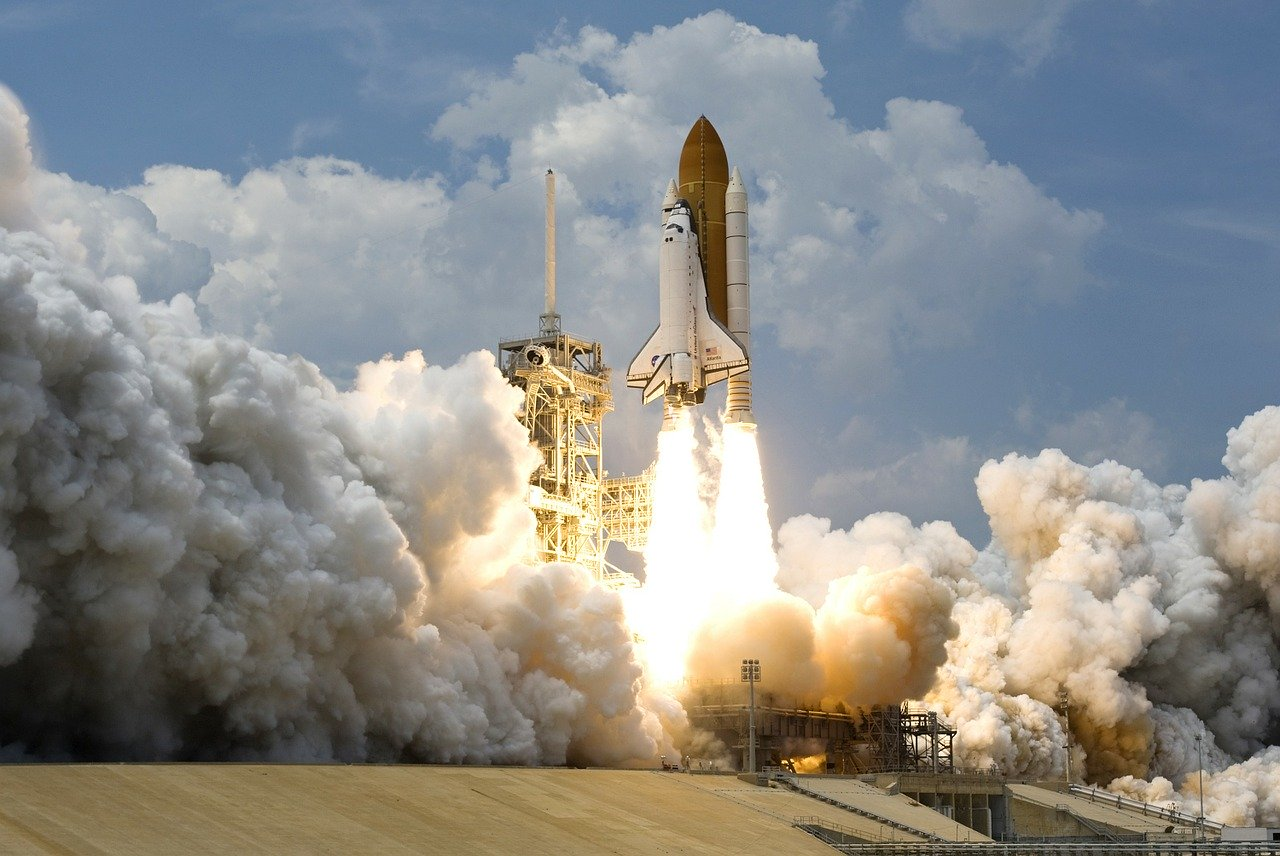
\includegraphics[scale=.2]{../figures/fig1.jpg}
\caption{Rocket Launch imaged using a visible camera}
\label{fig_rocket}
\end{figure}

In Figure \ref{fig_rocket}, a photo of the rocket launch using visible camera.

\subsection{Modelling}
Here the first equation of the model :
\begin{equation}
\frac{\partial T}{\partial t}=\frac{1}{a}\frac{\partial^2 T}{\partial x^2},
\label{eq_chaleur}
\end{equation}
where $a$ is the thermal diffusivity. In equation \ref{eq_chaleur}, $x$ stands for the spatial coordinate.

\subsection{Inverse processing}
Quod cum ita sit, paucae domus studiorum seriis cultibus antea celebratae nunc ludibriis ignaviae torpentis exundant, vocali sonu, perflabili tinnitu fidium resultantes. denique pro philosopho cantor et in locum oratoris doctor artium ludicrarum accitur et bybliothecis sepulcrorum ritu in perpetuum clausis organa fabricantur hydraulica, et lyrae ad speciem carpentorum ingentes tibiaeque et histrionici gestus instrumenta non levia.
\section{Results and discussion}
Structure:
\begin{enumerate}
\item	Statements of experimental results (including statistical analysis if appropriate); 
\item	Theoretical conclusions; 
\item	Discussion of results: interpretation; limitations, if any; comments on the techniques used and any problems encountered. 
\end{enumerate}

Tenses: present (description of the results and discussion) and preterit (description of the objectives which have been fulfill)

\section{Conclusions}
Structure:
\begin{enumerate}
\item	An overview of the results; 
\item A brief mention of the limitations of the work; 
\item A brief mention of possible applications; 
\item A brief mention of possible future work. 
\end{enumerate}

Tenses: present (description of the conclusion) and future (future work)


\section*{Acknowledgement}
Quod cum ita sit, paucae domus studiorum seriis cultibus antea celebratae nunc ludibriis ignaviae torpentis exundant, vocali sonu, perflabili tinnitu fidium resultantes. denique pro philosopho cantor et in locum oratoris doctor artium ludicrarum accitur et bybliothecis sepulcrorum ritu in perpetuum clausis organa fabricantur hydraulica, et lyrae ad speciem carpentorum ingentes tibiaeque et histrionici gestus instrumenta non levia.
\clearpage
\bibliographystyle{plain}
\bibliography{biblio} 

%----------------------------END OF EDIT-----------------------------------------------------------------------------------------
\end{document}